\documentclass[10pt,a4paper]{article}
\usepackage[margin=2.2cm]{geometry}
\usepackage{fontspec}
\usepackage{kotex}
\setmainfont{Apple SD Gothic Neo}
\setsansfont{Apple SD Gothic Neo}
\usepackage{amsmath,amssymb}
\usepackage{graphicx}
\usepackage{booktabs}
\usepackage{caption}
\usepackage[dvipsnames]{xcolor}
\usepackage[colorlinks=true,linkcolor=MidnightBlue,citecolor=MidnightBlue,
            urlcolor=MidnightBlue]{hyperref}
\usepackage{titlesec}
\titleformat{\section}{\large\bfseries}{\thesection}{0.6em}{}
\titleformat{\subsection}{\normalsize\bfseries}{\thesubsection}{0.5em}{}
\captionsetup{font=small,labelfont=bf}
\setlength{\parskip}{0.35em}
\setlength{\parindent}{0pt}

\usepackage{mdframed}
\newmdenv[linewidth=0.4pt,linecolor=gray!60,backgroundcolor=gray!5,
          innertopmargin=6pt,innerbottommargin=6pt,skipabove=8pt,skipbelow=8pt]{claimbox}
\newcommand{\claim}[2]{\begin{claimbox}\textbf{주장.} #1\par\smallskip
  \textcolor{gray!70}{\textbf{반증 조건.} #2}\end{claimbox}}

\title{\bfseries 두 왕국\\[2pt]
\large 전이의 땅과 사전의 땅 --- 다섯 도메인이 전부 $2\sigma$ 밖으로 갈렸다}
\author{월드모델 실험실 · 노트 $803$}
\date{2026-08-07}
\begin{document}\maketitle

\section{한 줄}

사용자가 문헌 로드맵을 가져왔다 --- \emph{TabPFN(SCM 합성 사전학습 · 문맥 내
베이즈)이 $n{=}80{\sim}600$ 레짐의 중앙 엔진 후보다.} 환경이 이미 서 있어서
(tabpfn $2.2.1$ · torch $2.8$) \textbf{같은 자료 · 같은 갈림 · 같은 유보행}으로
바로 쟀다. 얇은 도메인 다섯, $X = [A|M|t]$(챔피언이 보는 것과 같은 정보), 씨앗 $4$.

\begin{center}
\begin{tabular}{lrrrl}
\toprule
도메인(학습행) & 챔피언(합동) & TabPFN(단독) & 차 & 승자($2\sigma$ 밖) \\
\midrule
팝업($24$) & $0.3913$ & $0.1754$ & $-0.2159$ & 챔피언 \\
도서($80$) & $0.3838$ & $0.1704$ & $-0.2134$ & 챔피언 \\
게임($259$) & $0.6594$ & $0.5371$ & $-0.1223$ & 챔피언 \\
\textcolor{BrickRed}{아이돌($122$)} & $0.4613$ & $\mathbf{0.6311}$ & $\mathbf{+0.1698}$ & \textcolor{BrickRed}{\textbf{TabPFN}} \\
\textcolor{BrickRed}{시장팝업($123$)} & $0.1432$ & $\mathbf{0.2341}$ & $\mathbf{+0.0909}$ & \textcolor{BrickRed}{\textbf{TabPFN}} \\
\midrule
가중($585$유보) & $\mathbf{0.4244}$ & $0.3377$ & $-0.0867$ & \\
\bottomrule
\end{tabular}
\end{center}

\textbf{판정 (다) --- 판 중앙 엔진으로서의 TabPFN 은 기각.} 그러나 \textbf{다섯 중
다섯이 $2\sigma$ 밖으로 갈렸고 방향이 둘이다} --- 비김이 하나도 없다.

\begin{figure}[t]\centering
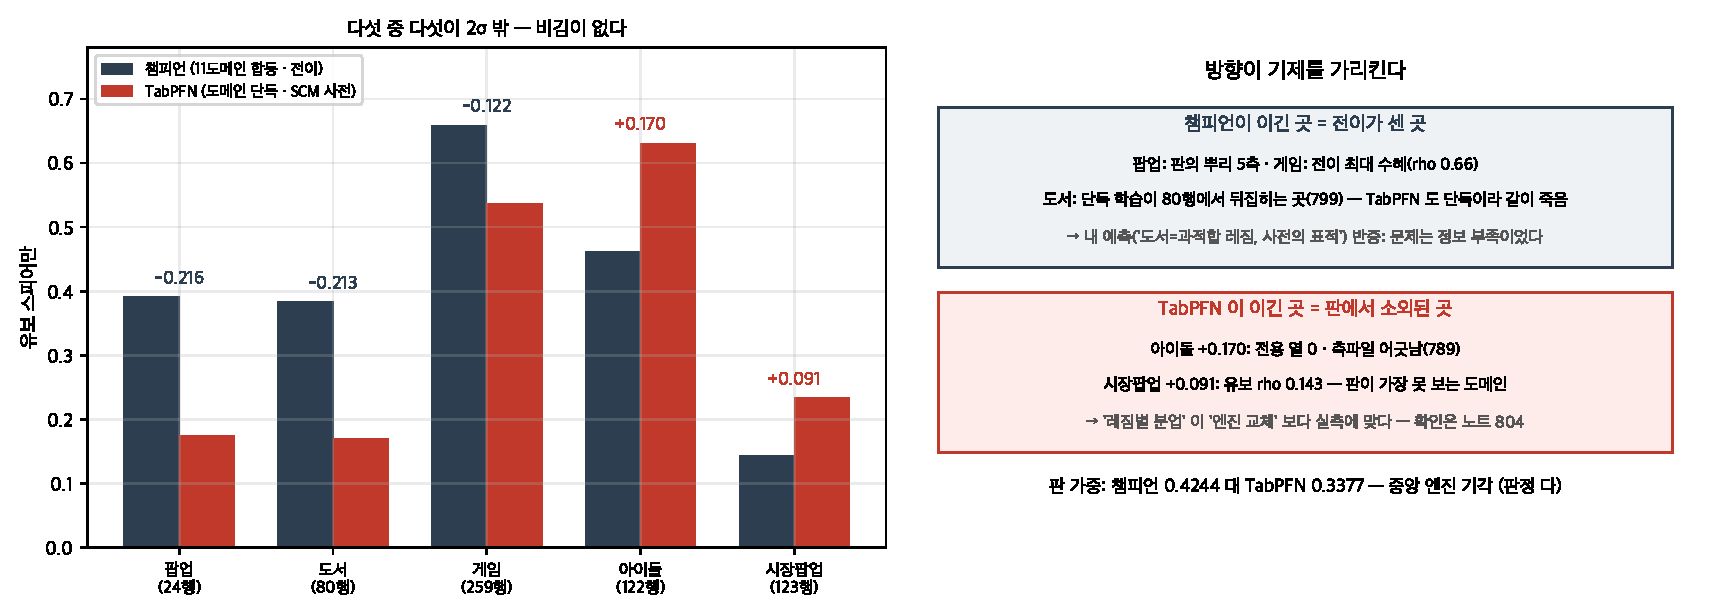
\includegraphics[width=0.92\textwidth]{figs/two.pdf}
\caption{왼쪽: 다섯 도메인 전부 $2\sigma$ 밖. 오른쪽: 갈린 방향이 기제를 가리킨다.}
\end{figure}

\section{방향이 기제를 가리킨다}

\claim{\textbf{챔피언이 이긴 곳은 전이가 센 곳이고, TabPFN 이 이긴 곳은 판에서
소외된 곳이다.} 팝업은 판의 뿌리 $5$축, 게임은 전이 최대 수혜(rho $0.66$), 도서는
단독 학습이 $80$행에서 뒤집히는 곳(논문 $163$)이라 \textbf{단독인 TabPFN 도 같이
죽었다}($0.1704$). 반대로 아이돌(전용 열 $0$ · 축파일 어긋남)과 시장팝업(유보
rho $0.143$ --- 판이 가장 못 보는 도메인)에서는 \textbf{합동 적합이 주는 것이
없어서 SCM 사전이 이겼다.} 사용자 로드맵의 두 논지 중 \emph{``레짐별 분업''}이
\emph{``중앙 엔진 교체''}보다 실측에 맞는다.}
{아이돌·시장팝업은 \textbf{결과를 보고 고른 둘}이다 --- 노트 $804$ 를 등록했다
(목록 못박음 · 새 씨앗 $4{\sim}7$). 확인되면 T$1$ 이 재개되고 ``소외 도메인 보조
헤드''가 챌린저 장부에 상설된다. \textbf{서빙 교체는 아니다.}}

\subsection*{내 예측이 반증된 자리가 가장 배울 곳이다}

나는 \emph{``도서($80$행)는 과적합 레짐이라 SCM 사전의 표적''}에 $60\%$ 를 걸었다.
\textbf{챔피언이 $-0.2134$ 로 압승했다.}

\claim{\textbf{도서의 문제는 과적합이 아니라 정보 부족이고, 전이가 그것을 메운다.}
논문 $163$(도서 열이 해로움)과 이번(단독 TabPFN 도 죽음)이 같은 곳을 가리킨다 ---
$80$행짜리 도메인은 \emph{자기 자료만으로는} 어떤 모형으로도 안 된다. 사전은
공짜 정보가 아니다 --- \textbf{SCM 사전은 ``세계가 대체로 어떤가''를 주지 ``이
도메인이 어떤가''를 주지 않는다.} 후자는 이웃 도메인의 전이가 준다.}
{그러면 아이돌은 왜 반대인가 --- 아이돌도 $122$행이다. 차이 후보는 \textbf{전이의
질}(아이돌은 축파일 어긋남 · 전용 열 $0$)이지만 \textbf{안 갈랐다.} 확인(노트
$804$) 후 아이돌의 축 배선을 고치면 챔피언이 따라잡는지가 가르는 시험이다.}

\section{규칙 반성 --- 셋째 갈래 상호작용}

내 갈래는 ``어느 쪽이 이기나''로 짜였다: (가) TabPFN $\geq 2$ 승 \emph{이고}
가중 승 · (다) 챔피언 $\geq 2$ 승. \textbf{실측은 ``둘 다 자기 구역에서 이긴다''}
--- (가)의 반쪽과 (다)가 동시에 참이고, 가중 조건이 아이돌·시장팝업의 발견을
판정문에서 가릴 뻔했다. 규약 $46$ 이 경고한 자리의 셋째 사례로 적는다.

\section{로드맵의 나머지와 이 실험실의 자리}

사용자 스택(동결 임베딩 병기 · TabPFN 헤드 · 랭킹 헤드 · 시장층 PCMCI · DML ·
운영 마이크로 RCT)에서 \textbf{이번 측정이 답한 것}: B$1$ 은 중앙이 아니라 소외
도메인 보조가 맞다(확인 대기). \textbf{다음 측정 후보로 올린 것}: A$1$ 동결 임베딩
병기(T$1$ 다음 실험 · 같은 챌린저 장부 · 리더보드 불신 조항 포함). \textbf{수집
기준 전환}(``라벨이 공공이고 조밀한 것'')은 T$7$ 에 우선순위로 새겼다 --- KOBIS
가 첫째이고 \textbf{사람 행동(키 발급)이 문이다.}

\end{document}
